% use the answers clause to get answers to print; otherwise leave it out.
\documentclass[11pt,addpoints,answers]{exam}
%\documentclass[11pt,addpoints]{exam}
\RequirePackage{amssymb, amsfonts, amsmath, latexsym, verbatim, xspace, 
setspace, wasysym, mathrsfs}
\usepackage{graphicx}

% By default LaTeX uses large margins.  This doesn't work well on exams; problems
% end up in the "middle" of the page, reducing the amount of space for students
% to work on them.
\usepackage[margin=1in]{geometry}
\usepackage{enumerate}
\usepackage[hidelinks]{hyperref}

% Here's where you edit the Class, Exam, Date, etc.
\newcommand{\class}{NPRE 560}
\newcommand{\term}{Fall 2024}
\newcommand{\assignment}{HW 4}
\newcommand{\duedate}{2024.11.18}
%\newcommand{\timelimit}{50 Minutes}
\newcommand{\StudentName}{Oleksandr Yardas} %Please include your name here

\newcommand{\nth}{n\ensuremath{^{\text{th}}} }
\newcommand{\ve}[1]{\ensuremath{\mathbf{#1}}}
\newcommand{\Macro}{\ensuremath{\Sigma}}
\newcommand{\vOmega}{\ensuremath{\hat{\Omega}}}

% For an exam, single spacing is most appropriate
\singlespacing
% \onehalfspacing
% \doublespacing

% For an exam, we generally want to turn off paragraph indentation
\parindent 0ex

%\unframedsolutions

\begin{document} 

% These commands set up the running header on the top of the exam pages
\pagestyle{head}
\firstpageheader{}{}{}
\runningheader{\class}{\assignment\ - Page \thepage\ of \numpages}{Due \duedate}
\runningheadrule

\class \hfill \StudentName \hfill \term \\
\assignment \hfill Due \duedate\\
\rule[1ex]{\textwidth}{.1pt}
%\hrulefill

%%%%%%%%%%%%%%%%%%%%%%%%%%%%%%%%%%%%%%%%%%%%%%%%%%%%%%%%%%%%%%%%%%%%%%%%%%%%%%%%%%%%%
%%%%%%%%%%%%%%%%%%%%%%%%%%%%%%%%%%%%%%%%%%%%%%%%%%%%%%%%%%%%%%%%%%%%%%%%%%%%%%%%%%%%%
\begin{itemize}
        \item Show your work. 
        \item This work must be submitted online as a \texttt{.pdf} through Canvas.
        \item Work completed with LaTeX or Jupyter earns 1 extra point. Submit 
                source file (e.g. \texttt{.tex} or \texttt{.ipynb}) along with 
                the \texttt{.pdf} file.
        \item If this work is completed with the aid of a numerical program 
                (such as Python, Wolfram Alpha, or MATLAB) all scripts and data 
                must be submitted in addition to the \texttt{.pdf}.
        \item If you work with anyone else, document what you worked on together.
\end{itemize}
\rule[1ex]{\textwidth}{.1pt}

% ---------------------------------------------
\begin{questions}
        % ---------------------------------------------
        \question (Hetrick 6-3, 6-4, 6-5, 6-6, 6-7, 6-8) Below, G(s)H(s) is the open-loop transfer function. For each, 
        plot the stable region for the closed-loop system in the $K(\alpha)$ 
        plane.
        \begin{parts}
            Poles of the closed-loop transfer function, $Y(s)$, characterize the
            stability of the system. If the poles of $Y(s)$ are in the
            left-hand half of the complex plane. An equivalent condition is
            that the roots of the characteristic equation
            $D(s)=P_{G}(s)P_{H}(s) + D_{G}(s) D_{H}(s)$ are all negative and
            real. This in turn, is equivalent to the condition than all of the
            Routh numbers of the characteristic polynomial are positive, that
            is, all of the numbers in first column of the Routh array are
            positive. If $D(s)$ has the form
            \[
                D(s) = a_{n}s^{n} + a_{n-1}s^{n-1} + a_{n-2}s^{n-2} +
                a_{n-3}s^{n-3} +\ldots 
            \]
            then the Routh array is given by 
            \[
            \begin{matrix}
                a_n & a_{n-2} & \ldots\\
                a_{n-1} & a_{n-3} & \ldots\\
                b_1 & \ldots & \\
            \end{matrix}
            \]
            where the Routh numbers are the first column of this array. The
            last Routh number is $a_{0}$, which is appended to the end of the
            first column. $b_1$ is given by
            \[
                b_1 = a_{n-2} - \frac{a_{n}a_{n-3}}{a_{n-1}}
            \]
            In practice, we form $D(s)$ by taking the sum of the
            numerator and the denominator of $G(s)H(s)$
                \part[5] $G(s)H(s) = \frac{K}{(s+2)(s+\alpha)}$
                \begin{solution}
                    $D(s) = s^{2} + (2 + \alpha)s + 2\alpha + K$. We don't need
                    to calculate $b_1$ since $a_{n-3} = 0$. So our Routh array is 
                    \[
                    \begin{matrix}
                        1\\
                        2 + \alpha\\
                        2\alpha + K
                    \end{matrix}
                    \]
                    So the region of stability is for $\alpha > -2$ and $K > -2
                    \alpha$:
                    \begin{center}
                        \centering
                        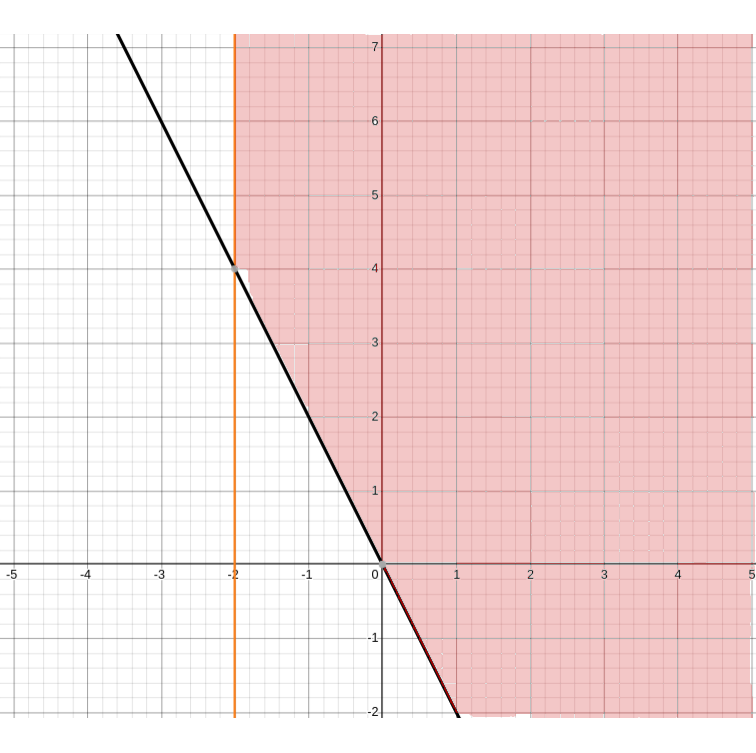
\includegraphics[width=0.5\textwidth]{figs/case-a.png}
                    \end{center}
                    %% PLOT
                \end{solution}
                \part[5] $G(s)H(s) = \frac{K + \alpha}{(s+2)(s+\alpha)}$
                \begin{solution}
                    $D(s) = s^{2} + (2 + \alpha)s + 3\alpha + K$. Again,
                    $a_{n-3}=0$ so we can immediately get out Routh numbers:
                    \[
                    \begin{matrix}
                        1\\
                        2 + \alpha\\
                        3\alpha + K
                    \end{matrix}
                    \]
                    So the region of stability is for $\alpha > -2$ and $K > -3
                    \alpha$:
                    %%plot
                    \begin{center}
                        \centering
                        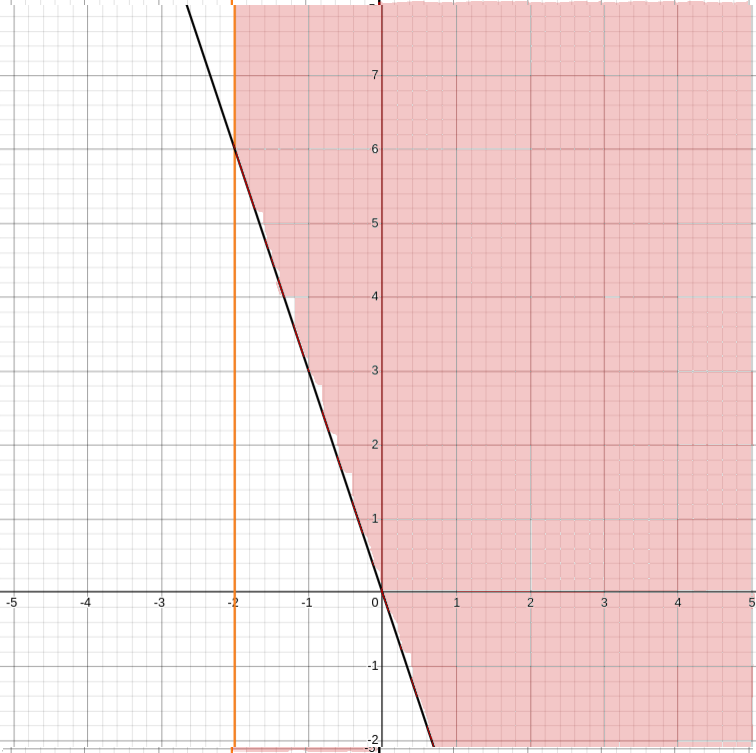
\includegraphics[width=0.5\textwidth]{figs/case-b.png}
                    \end{center}

                \end{solution}
                \part[5] $G(s)H(s) = \frac{K\alpha}{(s+2)(s+\alpha)}$
                \begin{solution}
                    $D(s) = s^{2} + (2 + \alpha)s + \alpha(2 + K)$. Again,
                    $a_{n-3}=0$ so we can immediately get out Routh numbers:
                    \[
                    \begin{matrix}
                        1\\
                        2 + \alpha\\
                        \alpha(K + 2)
                    \end{matrix}
                    \]
                    So the region of stability is for $\alpha > -2$ and $K > -2$
                    %% plot
                    \begin{center}
                        \centering
                        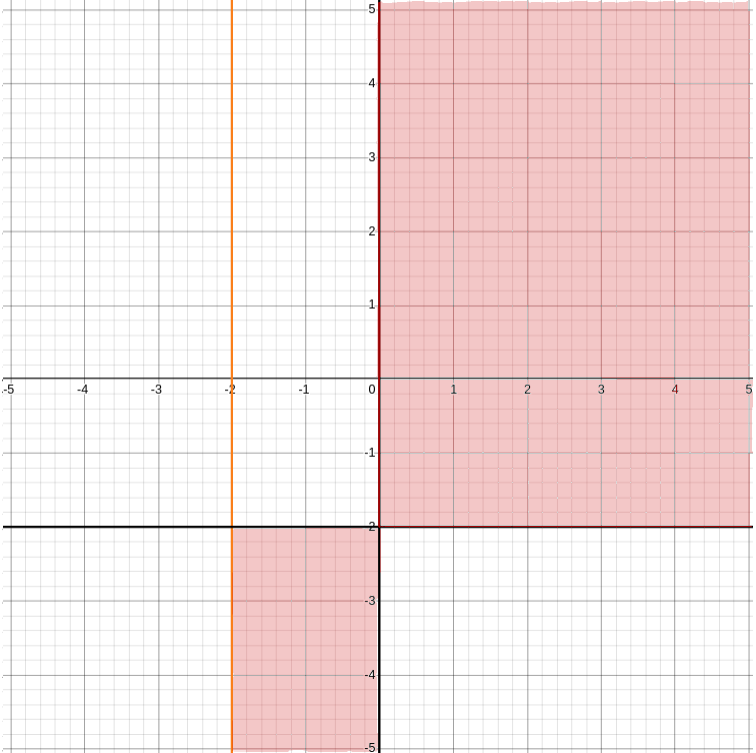
\includegraphics[width=0.5\textwidth]{figs/case-c.png}
                    \end{center}

                \end{solution}
                \part[5] $G(s)H(s) = \frac{K + \alpha}{(s+2)^2(s+\alpha)}$
                \begin{solution}
                    $D(s) = s^{3} + (4 + \alpha)s^{2} + 4(1+\alpha)s + 5\alpha +
                    K$, so $b_{1} = 4(1+\alpha) - \frac{5\alpha + K}{4 +
                    \alpha}$
                    The Routh array is then
                    \[
                    \begin{matrix}
                        1 & 4(1+\alpha)\\
                        4+\alpha & 5\alpha + K \\
                        4(1+\alpha) - \frac{5\alpha + K}{4 +
                    \alpha} & 0 \\
                        5\alpha + K & 
                    \end{matrix}
                    \]
                    So the region of stability is $\alpha > -4$, $K <
                    4\alpha^{2} + 15\alpha + 16$, and $K > 5\alpha$
                    %% PLOT
                    \begin{center}
                        \centering
                        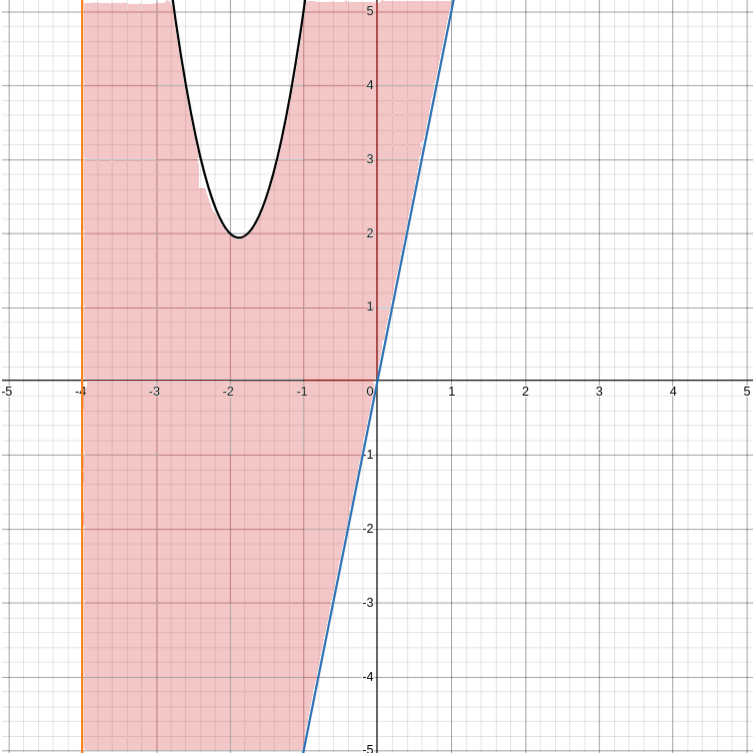
\includegraphics[width=0.5\textwidth]{figs/case-d.png}
                    \end{center}

                \end{solution}
                \part[10] $G(s)H(s) = \frac{K + \alpha}{(s-1)(s+2)(s+\alpha)}$
                \begin{solution}
                    $D(s) = s^3 + (alpha + 1)s^{2} + (\alpha - 2) s - \alpha +
                    K$, so $b_1 = \alpha - 2 - \frac{K-\alpha}{\alpha + 1}$. The
                    Routh array is then
                    \[
                    \begin{matrix}
                        1 & \alpha - 2\\
                        1+\alpha & K - \alpha \\
                        \alpha-2 - \frac{K- \alpha}{\alpha + 1} & 0 \\
                        K - \alpha & 
                    \end{matrix}
                    \]
                    So the region of stability is $\alpha > -1$, $K>\alpha$, and
                    $K < \alpha^{2} - 2$.
                    %%PloT
                    \begin{center}
                        \centering
                        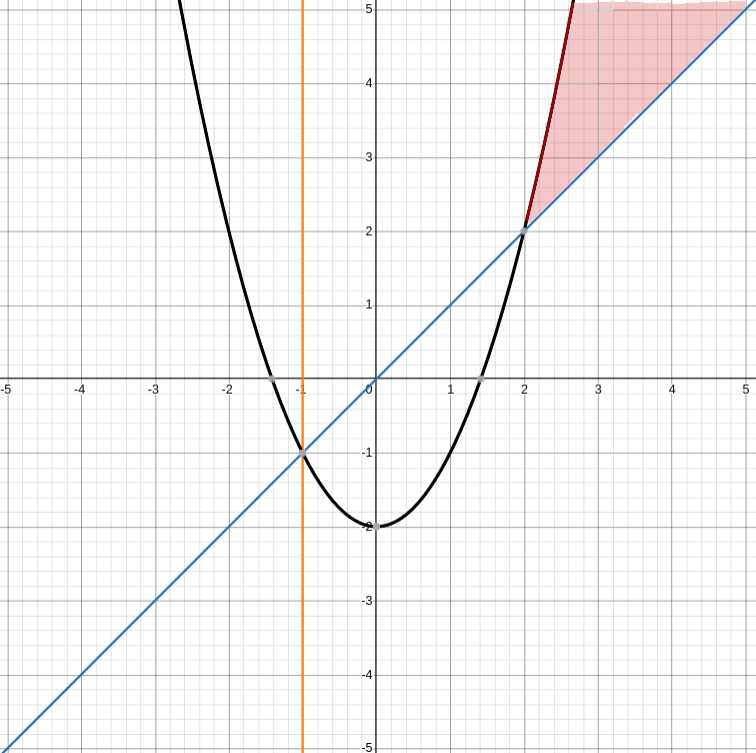
\includegraphics[width=0.5\textwidth]{figs/case-e.png}
                    \end{center}

                \end{solution}
                \part[10] $G(s)H(s) = \frac{K(s+1)}{(s-1)(s+2)(s+\alpha)}$
                \begin{solution}
                    $D(s) = s^3 + (\alpha + 1)s^{2} + (K + \alpha - 2) s - 2\alpha +
                    K$, so $b_1 = K + \alpha - 2 - \frac{K-2\alpha}{1 +
                    \alpha}$. The Routh array is then
                    \[
                    \begin{matrix}
                        1 & K + \alpha - 2 \\
                        \alpha + 1 & K - 2\alpha \\
                        K + \alpha - 2 - \frac{K-2\alpha}{1 +
                        \alpha} & 0\\
                        K - 2\alpha &
                    \end{matrix}
                    \]
                    
                    So the region of stability is $\alpha > -1$, $K > 2\alpha$,
                    and $K > \frac{2}{\alpha} - \alpha - 1$
                    \begin{center}
                        \centering
                        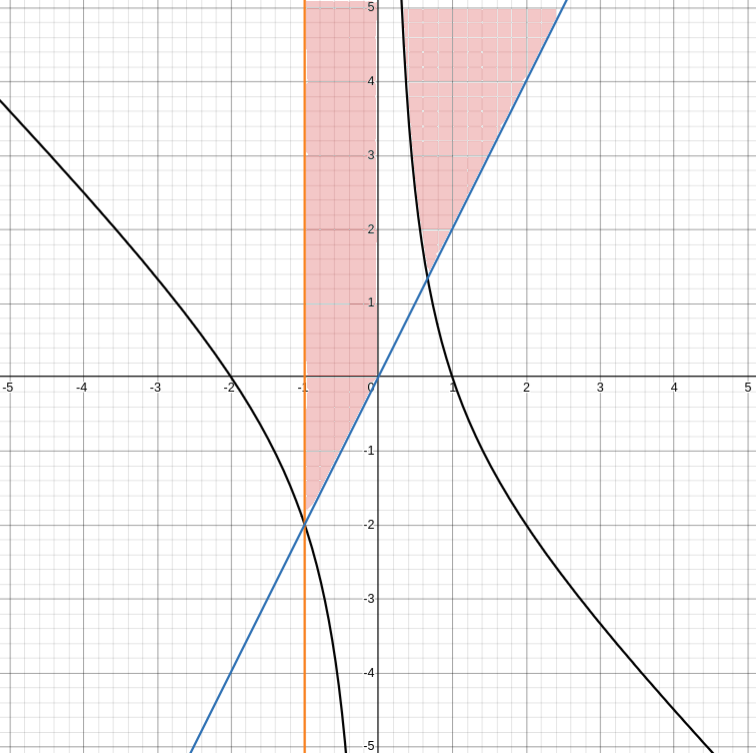
\includegraphics[width=0.5\textwidth]{figs/case-f.png}
                    \end{center}

                \end{solution}
        \end{parts}
        % ---------------------------------------------
        \question[20] (D\&H 6-26) Explicitly perform the Laplace transform 
        inversion of the zero power transfer function, $Z(s)$ to obtain the 
        impulse response function $\mathscr{Z}(t)$.
                \begin{solution}
                        solution here
                \end{solution}
       
        % ---------------------------------------------
        \question[30] (D\&H 6-23) Calculate the amplitude and phase angle for the 
        zero power transfer function and plot these as functions of frequency. 
        Assume one group of delayed neutrons with $\beta = 0.0065$, $\lambda = 
        0.08s^{-1}$, and $\Lambda = 10^{-4}s$.
                \begin{solution}
                    The one-group zero-power transfer function is
                    \[
                        Z(s) = \frac{1}{s}\left[\Lambda + \frac{\beta}{s +
                        \lambda}\right]
                    \]
                    From D\&H 6.II.D.3, we have that the amplitude is
                    $|Z(i\omega)| = \sqrt{\text{Re}^{2}[Z(i\omega)] +
                    \text{Im}^{2}[Z(i\omega)]}$, and the phase angle is given by
                    $\arctan(\frac{\text{Im}[Z(i\omega)]}{\text{Re}[Z(i\omega)]
                    })$. In the context of complex numbers, this is sometimes
                    called the $\text{arg}$ function or the $\arctan 2$
                    function.

                    Plots of the magnitude and phase angle are below:

                    \begin{center}
                        \centering
                        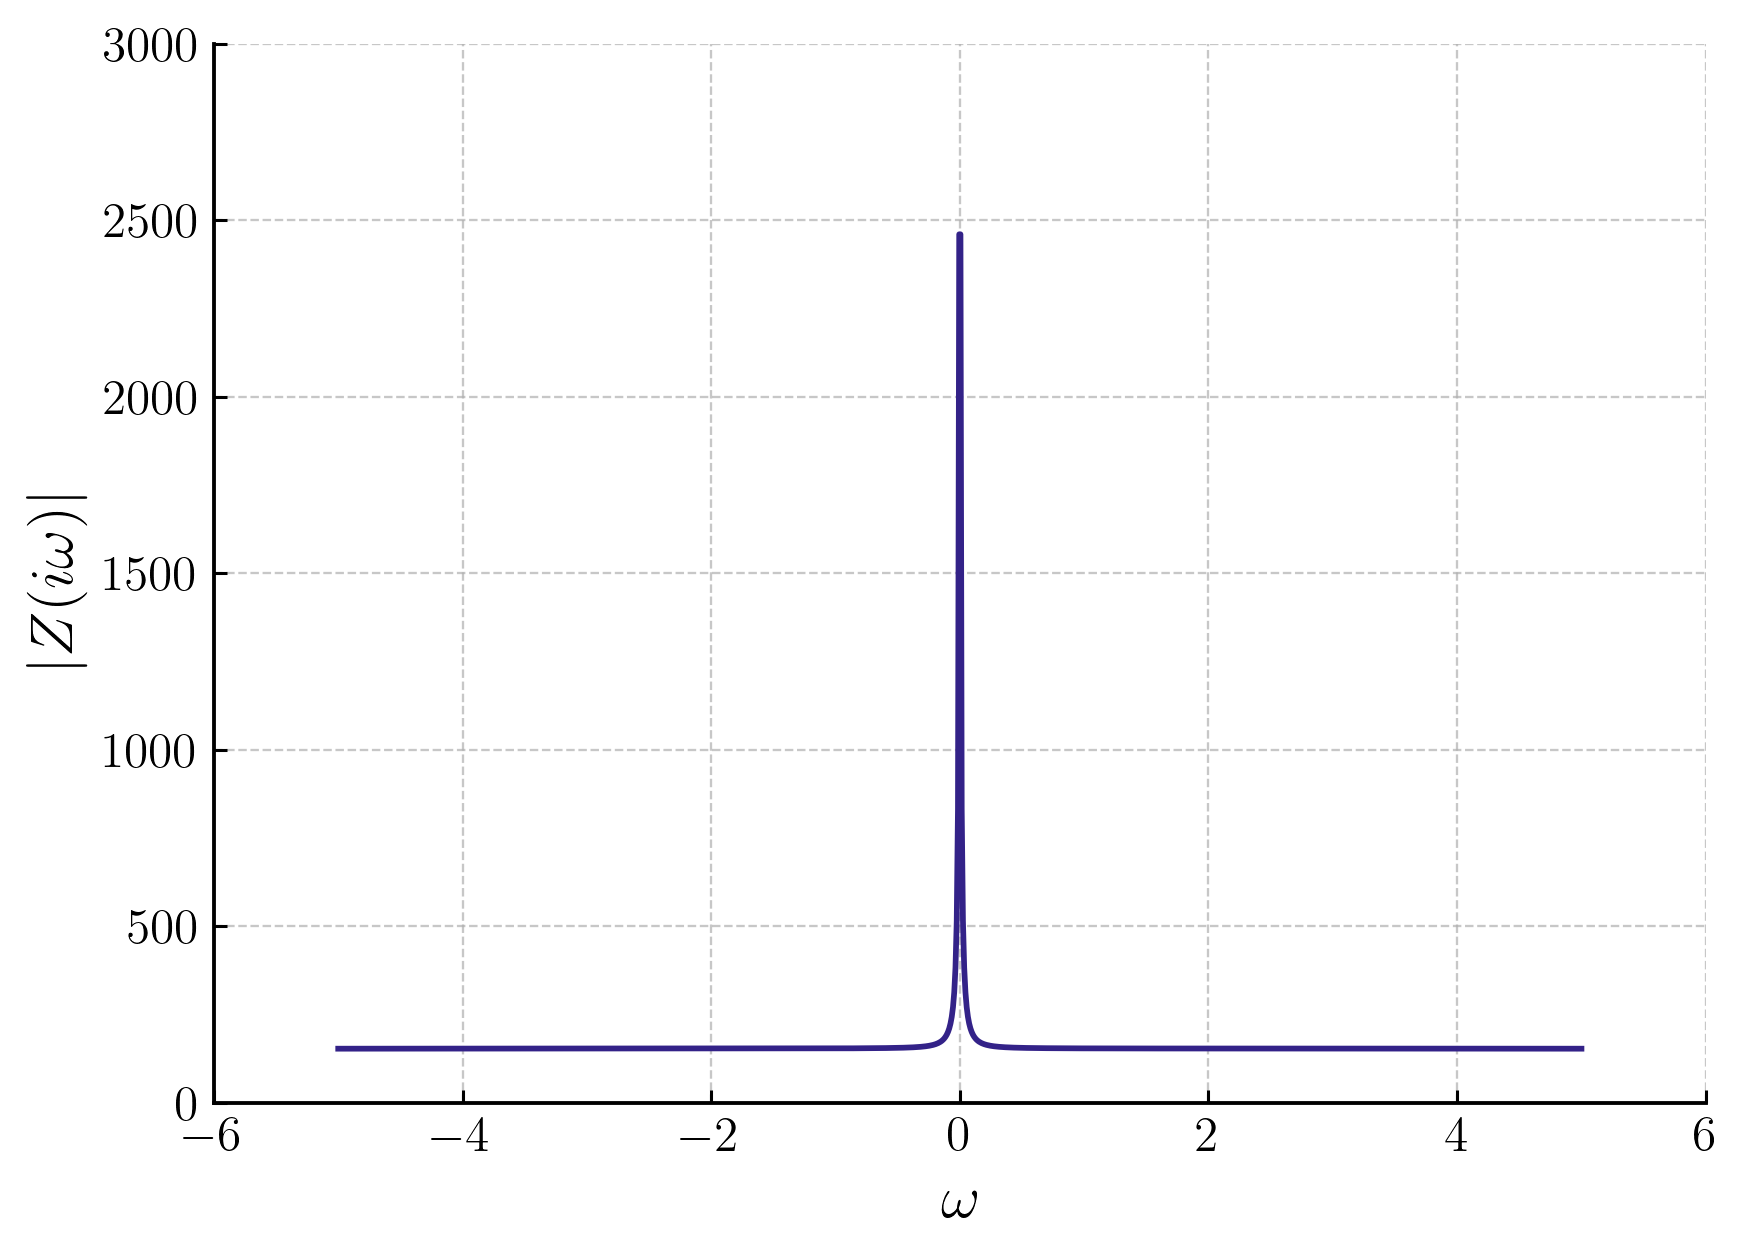
\includegraphics[width=0.5\textwidth]{figs/magnitude.png}
                    \end{center}
                    \begin{center}
                        \centering
                        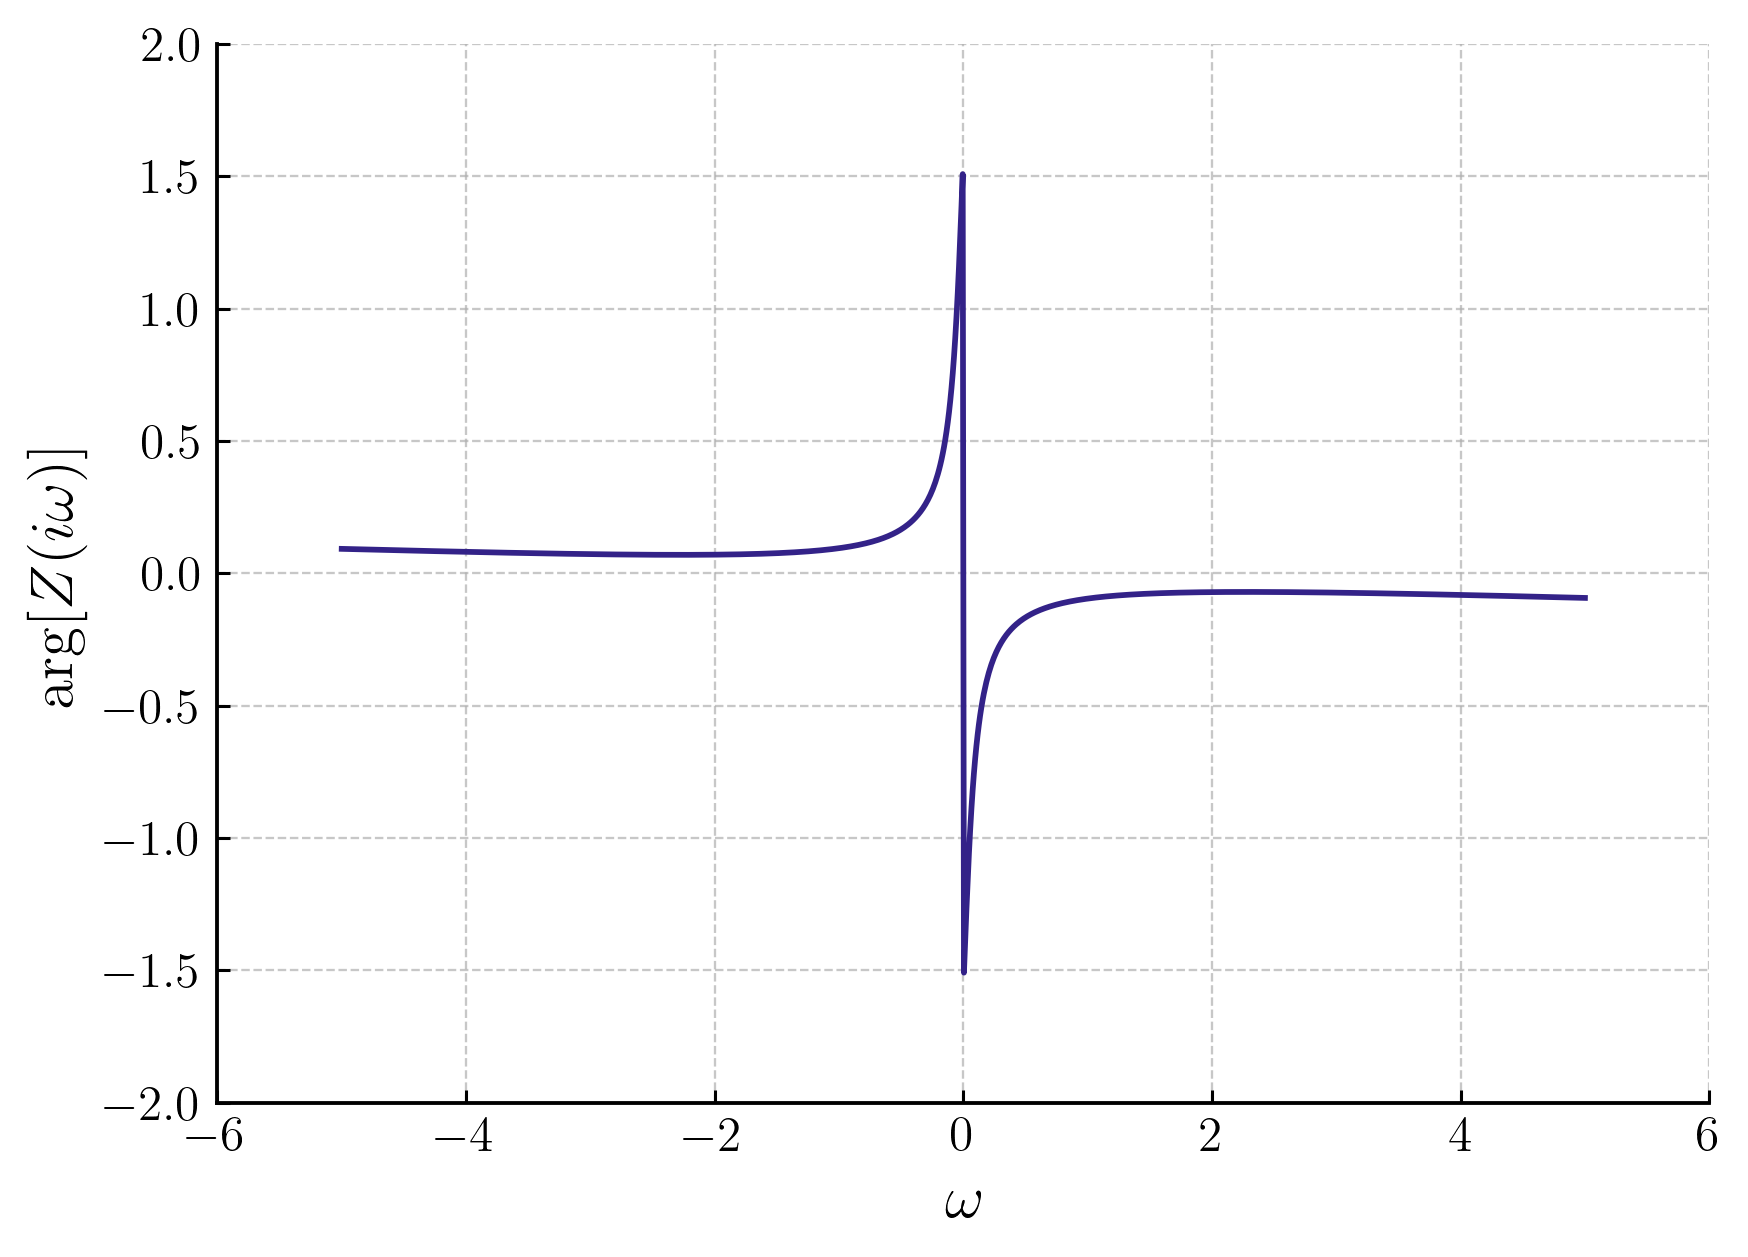
\includegraphics[width=0.5\textwidth]{figs/phase.png}
                    \end{center}



                \end{solution}
       
        % ---------------------------------------------
        \question[10] (D\&H 6-32) In a prompt critical reactor excursion, a 
        large amount of reactivity (measured above prompt critical) $\rho_0$ is 
        instantaneously inserted in an equillibrium reactor at $t=0$. Assume 
        that:
        \begin{itemize}
                \item the effect of delayed neutrons is negligible on the time 
                        scales under consideration.
                \item the reactor shuts itself down by thermal expansion of the 
                        core in such a way that negative reactivity is 
                        ``added'' proportional to the total heat energy 
                        generated up to time $t$. That is, $\rho = \rho_0 - 
                        \gamma\int_0^t{P(t')dt'}$. 
        \end{itemize}

        Find the power level $P(t)$  where $t$ is measured from the time of 
        reactivity insertion, and is measured in units of the prompt neutron lifetime.
        [This is known as the Fuchs-Hansen model of reactor excursion.]

        {\bf SOLUTION:} (The \verb.solution. environment was cutting off my
        answer, so I'm doing it out of the environment)
                    In the prompt case neglecting delayed neutrons, our point
                    reactor kinetic equation is simply
                    \[
                        \frac{dP}{dt} = \frac{\rho(t)}{\Lambda} P(t)
                    \]
                    Expanding $\rho(t) = \rho_0 - \gamma \int_{0}^{t} P(t')dt'$,
                    we get
                    \begin{equation}
                        \label{eq:prk-base}
                        \frac{dP}{dt} = \left[\frac{\rho_0}{\Lambda} -
                        \frac{\gamma}{\Lambda}\int_{0}^{t}P(t') dt'\right] P(t)
                    \end{equation}
                    Now, letting $a \equiv \frac{p_0}{\Lambda}$ and $b \equiv
                    \frac{\gamma}{\Lambda}$, define $y(t) = a -
                    b\int_{0}^{t}P(t') dt'$. We can then rewrite Equation
                    \ref{eq:prk-base} as
                    \begin{equation}
                        \label{eq:prk-y}
                        \frac{dP}{dt} = P(t)y(t)
                    \end{equation}

                    Now, notice that $\frac{dy}{dt} =
                    -bP(t)$, and $\frac{d^{2}y}{dt^{2}} = -b \frac{dP}{dt}$.
                    Substituting in Equation \ref{eq:prk-y} into the
                    $\frac{d^{2}y}{dt^{2}}$, and using $\frac{dy}{dt} = -bP(t)$,
                    we get
                    \[
                        \frac{d^{2}y}{dt^{2}} = y \frac{dy}{dt}
                    \]
                    Integrating both sides with resepect to $t$ yields
                    \[
                        \frac{dy}{dt} = \int y \frac{dy}{dt} dt
                    \]
                    Using integration by parts on the RHS, we get $\int y
                    \frac{dy}{dt} dt = \frac{1}{2}y^{2} + C$, where $C$ is some
                    constant. Since the constant is arbitrary, we can redefine
                    it as anything we want. Suppose we redefine the constant as
                    $-\frac{1}{2}c^{2}$. We then have that
                    \begin{equation}
                        \label{eq:y-c}
                        \frac{dy}{dt} = \frac{1}{2}(y^{2} - c^{2})
                    \end{equation}
                    to find $c$, note that $\frac{dy}{dt}\Big|_{t=0} = -bP_0 =
                    \frac{1}{2}(y(0)^{2} - c^{2})$.  Based on the definition of
                    $y(t)$, we have that $y(0) = a$, so we are left with the
                    equality $-bP_0 = \frac{1}{2}(a^{2} - c^{2})$. Solving for
                    $c$ yields
                    \[
                        c = \sqrt{a^{2} + 2bP_0} 
                    \]
                    Now, we have $y$ in a form that we cannot solve directly.
                    Let's reformulate $y$ in terms of another function $x(t)$:
                    \begin{equation}
                        \label{eq:y-x}
                        y(t) = \frac{1}{x(t)} + c
                    \end{equation}
                    Note that $x(0) = \frac{1}{a-c}$
                    Substituing this definition into Equation \ref{eq:y-c}, we
                    get
                    \[
                        -\frac{1}{x^{2}(t)}\frac{dx}{dt} =
                        \frac{1}{2}(\frac{1}{x^{2}} + 2cx(t))
                    \]
                    Rearranging terms yields
                    \[
                        \frac{dx}{dt} + cx = -\frac{1}{2}
                    \]
                    The homogenous part of the solution is $u(0)e^{-ct}$. The
                    non-homogenous part takes some guesswork but assuming
                    a solution of the form $A(1-e^{-ct})$ yields
                    $A=-\frac{1}{2c}$, so we have
                    \[
                        x(t) = \frac{1}{a-c}e^{-ct} - \frac{1}{2c}(1-e^{-ct}) 
                    \]
                    Which we can rearrange to
                    \[
                        x(t) = -\frac{1}{2c}(1+\frac{c+a}{c-a}e^{-ct}) 
                    \]
                    Interting this into Equation \ref{eq:y-x}, we get
                    \[
                        y(t) = -2c(1 + \frac{c+a}{c-a}e^{-ct})^{-1} + c
                    \]
                    Substituting this into $\frac{dy}{dt} = -bP(t)$, we get
                    \[
                        \frac{-2c^{2}Ae^{-ct}}{(1+Ae^{-ct})^{2}} = -bP(t)
                    \]
                    where $A\equiv \frac{c+a}{c-a}$. Solving for $P$, we get
                    \[
                        P(t) = \frac{2c^{2}Ae^{-ct}}{b(1+Ae^{-ct})^{2}}
                    \]
\end{questions}



%\bibliographystyle{plain}
%\bibliography{hw01}
\end{document}
